% Tests and convergence of the moment radiative transfer (M1, OTVET) and of the rays.
% A working document beside main.tex, not part of the paper. Figures: figures/convergence/,
% tables: data/convergence/, lead figure: scripts/fig_transfer_diffusion.py.
\documentclass[11pt]{article}
\usepackage[margin=1in]{geometry}
\usepackage{amsmath,amssymb}
\usepackage{graphicx}
\usepackage{booktabs}
\usepackage{xcolor}
\usepackage[authoryear,round,semicolon]{natbib}
\usepackage[colorlinks=true,linkcolor=blue,citecolor=blue,urlcolor=blue]{hyperref}

\providecommand{\mnras}{MNRAS}\providecommand{\apj}{ApJ}\providecommand{\apjs}{ApJS}\providecommand{\aj}{AJ}
\providecommand{\apjl}{ApJL}\providecommand{\aap}{A\&A}\providecommand{\jcap}{JCAP}
\providecommand{\pasp}{PASP}\providecommand{\araa}{ARA\&A}\providecommand{\prd}{Phys.~Rev.~D}
\providecommand{\nat}{Nature}\providecommand{\physrep}{Phys.~Rep.}\providecommand{\na}{New Astron.}
\newcommand{\chat}{\hat{c}}
\newcommand{\hmpc}{\,h\,\mathrm{Mpc}^{-1}}
\newcommand{\mpch}{\,h^{-1}\,\mathrm{Mpc}}
\newcommand{\xv}{x_{\rm V}}
\newcommand{\dx}{\Delta x}
\newcommand{\pending}[1]{\textcolor{red}{[pending: #1]}}

\begin{document}

\title{Tests and convergence of the moment radiative transfer}
\author{Working notes for the RT-closure paper}
\date{Draft of 2026-11-21}
\maketitle

\begin{abstract}
\noindent This document collects the tests of the M1 and OTVET solvers of the code and of the ray tracing they are
compared with. The central test is the transfer function between sources and photon density in a medium
of uniform mean free path, which has an exact solution and a linear solution for each closure, and for
which the numerical diffusion of the transport scheme can be modelled. Three results matter for the
paper. (i) Both solvers reproduce the linear solution of their closure where it is resolved. (ii) M1's
small-scale response is set by two numerical terms, the diffusion of the first-order flux and the
photons a source injects into its own cell; it converges slowly, about first order in the cell size. (iii) In
the reionization runs M1's excess of photoionization-rate power over the rays at small scales falls
with resolution as that predicts (a ratio of 3.1, 1.4 and 1.05 at $k=16\hmpc$ on $128^3$, $256^3$ and $512^3$ cells), while
its deficit at large scales after overlap, and OTVET's excess, do not go away.
The ray runs of the paper's suite are converged in ray number to 3\,\% at $k\ge2\hmpc$ and to 8--20\,\%
at $k\le1\hmpc$ after overlap.
\end{abstract}

\tableofcontents

%======================================================================
\section{The solver}\label{sec:solver}

The moment solver evolves the photon number density $N$ and flux $\mathbf F$ of each of five frequency
groups on the gas grid at the reduced speed of light $\chat$,
\begin{align}
\partial_t N + \chat\,\nabla\!\cdot\mathbf F &= S - \chat\kappa N, \label{eq:N}\\
\partial_t \mathbf F + \chat\,\nabla\!\cdot(\mathsf D N) &= -\chat\kappa\,\mathbf F, \label{eq:F}
\end{align}
with $\mathbf F$ in units of $\chat$. The two methods differ only in the Eddington tensor $\mathsf D$: M1
uses the local \citet{levermore84} form, and OTVET the optically thin tensor summed over the sources with
the minimum-image convention.

\paragraph{Transport.} The default scheme is the first-order global Lax--Friedrichs (GLF, Rusanov) flux with
wave speed $\chat$, unsplit in the three directions, as in ATON and RAMSES-RT \citep{aubert08,rosdahl13}.
One RT substep is one cell of light travel and is divided into $n_{\rm sub}=4$ subcycles (Courant number
$C=1/4$). After each subcycle $N\ge0$ and $|\mathbf F|\le N$ are enforced.

\paragraph{Sources and absorption.} Sources add photons isotropically to their own cell. Absorption,
photoheating and chemistry use the same routine as the rays, called once per substep with the
photon density in each cell. The order within a substep is a choice:
\begin{itemize}
\item \emph{inject after transport} (the default, \texttt{moment\_inject = 1}): the photons a source emits
in a substep are first exposed to absorption in their own cell and transported in the next substep;
\item \emph{inject before transport} (\texttt{moment\_inject = 0}): they are transported four subcycles
first, which moves most of them out of the source cell before anything absorbs them.
\end{itemize}

\paragraph{Second-order option.} A second-order scheme was added for this study (\texttt{moment\_order = 2}):
linear reconstruction of $N$, $\mathbf F$ and the group energy with the monotonized-central limiter, the GLF
flux of the two face states (each with the closure of its own state), and a two-stage Heun step. It needs
$C\le1/6$ and is 10--17 times more expensive in the transport.

%======================================================================
\section{Uniform mean free path: transfer function against the analytic solution}\label{sec:uniform}

\subsection{Set-up and the three reference curves}

The solver's own transport kernels are run to steady state in a periodic box of side $L$ with a fixed,
uniform mean free path $\lambda$: every substep ends with $N,\mathbf F\to N,\mathbf F\,e^{-\dx/\lambda}$ in place of the
chemistry. Sources of random luminosity $L_s$ are placed in every cell (or in a few cells). The measured
quantity is the transfer function
\begin{equation}
T(k)\equiv\left[\frac{P_N(k)}{P_L(k)}\right]^{1/2},
\end{equation}
normalised so that $T\to1$ as $k\to0$, and the cross-correlation coefficient $r(k)$ of $N$ with the
sources. With uniform opacity $\Gamma\propto N$, so $T$ is the transfer function of the photoionization
rate. This is the test of \citet{gnedin25}.

Throughout, $\kappa=1/\lambda$, the source field is $S(\mathbf x)=\bar S\,[1+\delta_L(\mathbf x)]$, and
$T=\delta_N(\mathbf k)/\delta_L(\mathbf k)$ with $\delta_N=N/\bar N-1$ and $\bar N=\bar S/(\chat\kappa)$.

\begin{enumerate}
\item \textbf{Exact.} In steady state each source contributes $L_s\,e^{-r/\lambda}/(4\pi r^2\chat)$ to $N$,
so $N$ is the source field convolved with that kernel. Its Fourier transform is
\begin{equation}
\frac{N(\mathbf k)}{S(\mathbf k)}=\frac{1}{\chat}\int_0^\infty\!dr\,e^{-r/\lambda}\,\frac{\sin kr}{kr}
=\frac{\arctan(k\lambda)}{\chat k},
\qquad\hbox{hence}\qquad
T_{\rm exact}(k)=\frac{\arctan(k\lambda)}{k\lambda}\label{eq:exact}
\end{equation}
\citep[][eq.~2]{gnedin25}, with $T\to1-k^2\lambda^2/3$ for $k\lambda\ll1$ and $T\to\pi/(2k\lambda)$ for
$k\lambda\gg1$.
\item \textbf{The closure, in the continuum.} In steady state and in Fourier space equations
(\ref{eq:N})--(\ref{eq:F}) are
\begin{equation}
i\mathbf k\cdot\mathbf F=S/\chat-\kappa N,\qquad i k_j\,(\mathsf D_{ij}N)=-\kappa F_i .\label{eq:steady}
\end{equation}
For M1 with many overlapping sources the state is nearly isotropic, $\mathsf D=\mathsf I/3$ to first
order in the perturbation, so $\mathbf F=-i\mathbf kN/3\kappa$ and
\begin{equation}
T_{\rm M1}(k)=\frac{1}{1+k^2\lambda^2/3}.\label{eq:m1lin}
\end{equation}
This is the diffusion limit. It agrees with equation (\ref{eq:exact}) to order $k^2\lambda^2$ and falls as
$3/(k\lambda)^2$ where the exact solution falls as $\pi/(2k\lambda)$: M1 has too little small-scale
structure once sources overlap.

For OTVET the tensor is not a function of the local state but of the source field,
$\mathsf D_{ij}(\mathbf x)=\sum_sL_s\hat n_i\hat n_j/r_s^2\,\big/\sum_sL_s/r_s^2$, and its perturbation
$\delta\mathsf D$ enters equation (\ref{eq:steady}) at first order through
$ik_j\,\delta\mathsf D_{ij}\bar N$. With $L_{\rm O}\equiv\int d^3r/r^2$ over the minimum-image cube
($=7.66\,L$),
\begin{equation}
\delta\mathsf D_{ij}(\mathbf k)=\frac{\delta_L(\mathbf k)}{L_{\rm O}}\int\!d^3r\,
\frac{\hat n_i\hat n_j-\delta_{ij}/3}{r^2}\,e^{-i\mathbf k\cdot\mathbf r}
=-\frac{\pi^2}{kL_{\rm O}}\left(\hat k_i\hat k_j-\frac{\delta_{ij}}{3}\right)\delta_L(\mathbf k),
\end{equation}
using $\int_0^\infty j_2(x)\,dx=\pi/4$ (the integral is taken to infinity, which holds for $kL\gg1$). Then
$k_ik_j\,\delta\mathsf D_{ij}=-(2\pi^2k/3L_{\rm O})\,\delta_L$ and
\begin{equation}
T_{\rm OTVET}(k)=\frac{1+2\pi^2k\lambda^2/(3L_{\rm O})}{1+k^2\lambda^2/3},\qquad L_{\rm O}=7.66\,L
\label{eq:otvetlin}
\end{equation}
\citep[eqs.~5.14--5.15 without the opacity response]{wu21}. The extra term is $0.86\,(k\lambda)(\lambda/L)$:
OTVET has too much structure when the mean free path approaches the box size, and for $k\lambda\gg1$ it
tends to $2\pi^2/(kL_{\rm O})$, which does not depend on $\lambda$.
\item \textbf{The closure with the scheme's numerical diffusion.} The first-order GLF flux through the
face between cells $i$ and $i+1$ is $\tfrac12(f_i+f_{i+1})-\tfrac12\chat\,(u_{i+1}-u_i)$ for a conserved
variable $u$ with physical flux $f$. Its difference across a cell is the centred difference of $f$ minus
$\tfrac12\chat\dx$ times the second difference of $u$: both moment equations acquire a diffusion term
$\tfrac12\chat\dx\nabla^2$. In equation (\ref{eq:steady}) this replaces $\mathbf k$ by the centred-difference
symbol $\mathbf s$ and $\kappa$ by $q$,
\begin{equation}
s_d=\frac{\sin k_d\dx}{\dx},\qquad
q=\kappa+\frac{1}{\dx}\sum_d(1-\cos k_d\dx)\;\simeq\;\kappa+\tfrac12k^2\dx,
\end{equation}
while the mean $\bar N=\bar S/(\chat\kappa)$ is unchanged, which leaves $\kappa$ in the numerator. The same
algebra then gives (for OTVET with $s_is_j\,\delta\mathsf D_{ij}\simeq-(2\pi^2|\mathbf s|^2/3kL_{\rm O})\,\delta_L$)
\begin{equation}
T^{\rm GLF}_{\rm M1}(\mathbf k)=\frac{\kappa}{q+|\mathbf s|^2/3q},\qquad
T^{\rm GLF}_{\rm OTVET}(\mathbf k)=\frac{\kappa+2\pi^2|\mathbf s|^2/(3qkL_{\rm O})}{q+|\mathbf s|^2/3q},
\label{eq:glf}
\end{equation}
which reduce to equations (\ref{eq:m1lin}) and (\ref{eq:otvetlin}) for $\dx\to0$. They are evaluated on
the grid's modes and averaged in the same $k$ bins as the measurement. For
$k\gtrsim(2/\lambda\dx)^{1/2}$ the numerical term dominates the flux equation, $|\mathbf s|^2/3q\to2/(3\dx)$,
and $T^{\rm GLF}_{\rm M1}$ flattens near $1.5\,\dx/\lambda$ instead of continuing as $3/(k\lambda)^2$.

For the second-order scheme, where its limiter is inactive (central slopes), the dissipation is a fourth
difference and the flux difference is a higher-order one. Equation (\ref{eq:glf}) holds with
\begin{equation}
q=\kappa+\frac{1}{8\dx}\sum_d(2-2\cos k_d\dx)^2\;\simeq\;\kappa+\tfrac18\dx^3\sum_dk_d^4,\qquad
s_d=\frac{\sin k_d\dx\,(3-\cos k_d\dx)}{2\dx}.\label{eq:muscl}
\end{equation}
\end{enumerate}

\subsection{The injection floor}\label{sec:floor}

One more term is needed for the default injection order: the photons a source emitted during the
current substep sit in its own cell when the photoionization rate is evaluated. This adds a white
component to $N$, which we call the \emph{injection floor}.

\paragraph{Derivation.} Let $\mathcal A$ be the transport of one substep (its $n_{\rm sub}$ subcycles), a
linear operator in the linear regime with Fourier symbol $A(\mathbf k)$; $A(0)=1$ because it conserves photons.
A substep of length $\Delta t=\dx/\chat$ injects $\Delta S=S\,\Delta t$ and ends with the absorption, which
multiplies $N$ and $\mathbf F$ by $1-f$,
\begin{equation}
f=1-e^{-\chat\Delta t/\lambda}=1-e^{-\dx/\lambda}.
\end{equation}
The two orders of operation are
\begin{align}
\hbox{inject after (default):}\quad & N\;\to\;\mathcal AN\;\to\;\mathcal AN+\Delta S\equiv N_1\;\to\;(1-f)\,N_1,\\
\hbox{inject before:}\quad & N\;\to\;N+\Delta S\;\to\;\mathcal A\,(N+\Delta S)\equiv N_0\;\to\;(1-f)\,N_0,
\end{align}
where $N_1$ and $N_0$ are the fields the chemistry sees. In steady state
$N_1=(1-f)\,\mathcal AN_1+\Delta S$ and $N_0=\mathcal A\,[(1-f)N_0+\Delta S]$, so mode by mode
\begin{equation}
N_1(\mathbf k)=\frac{\Delta S(\mathbf k)}{1-(1-f)A},\qquad N_0(\mathbf k)=A\,N_1(\mathbf k).\label{eq:n1n0}
\end{equation}
Both have the same mean, $\bar N=\Delta\bar S/f$ (which is $\bar S\lambda/\chat$ for $\dx\ll\lambda$), so the
transfer functions are
\begin{equation}
T_1=\frac{f}{1-(1-f)A},\qquad T_0=A\,T_1=\frac{fA}{1-(1-f)A},\label{eq:t1t0}
\end{equation}
and eliminating $A$ gives
\begin{equation}
T_1=(1-f)\,T_0+f=T_0+f\,(1-T_0).\label{eq:floor}
\end{equation}
Equation (\ref{eq:floor}) is exact for any linear transport operator, of either order: it uses only that
the two variants apply the same $\mathcal A$ and the same absorption. It can fail only through the nonlinear
parts of the solver (the M1 closure, the limiter of the second-order scheme, the realizability clamp). In the
code it holds to 1--4\,\% (below).

\paragraph{What it means.} The field the chemistry sees with the default order is the smoothed field of
the other order with weight $1-f$, plus the unsmoothed source field with weight $f$.
\begin{itemize}
\item \emph{It is a floor.} Where the transport has erased the structure ($A\to0$, $T_0\to0$), $T_1\to f$:
the photon density keeps a copy of the source field with amplitude $f\simeq\dx/\lambda$, at every $k$ up to the
Nyquist frequency. In the power spectrum this is a white term $f^2P_L$.
\item \emph{Injection before the transport smooths instead.} By equation (\ref{eq:t1t0}), $T_0=A\,T_1$: that
variant is the default one passed once more through a substep of transport, which spreads each source over
the cells its photons reach in the $n_{\rm sub}$ subcycles. The diffusion model of equation (\ref{eq:glf})
describes the semi-discrete steady state and contains no such factor, and the measured $T_0$ lies below it.
\item \emph{Where it matters.} The exact solution falls as $\pi/(2k\lambda)$, so the floor exceeds it for
\begin{equation}
k\dx>\frac{\pi}{2},
\end{equation}
independent of $\lambda$ and of the resolution, and is twice the exact $T$ at the Nyquist frequency
($k\dx=\pi$). The continuum M1 solution falls as $3/(k\lambda)^2$, so the floor exceeds it already for
$k>(3/\lambda\dx)^{1/2}$, close to the wavenumber $(2/\lambda\dx)^{1/2}$ at which the numerical diffusion takes
over. The two numerical terms therefore enter together and are of the same size: the diffusion plateau is
$\simeq1.5\,\dx/\lambda$ and the floor $\simeq\dx/\lambda$. Both are proportional to $\dx$ at fixed $k$;
the second-order scheme removes only the first.
\item \emph{It depends on the substep, not on the flux.} $f$ is the optical depth of the light travel between
two calls of the chemistry, $\chat\Delta t/\lambda$. A less diffusive flux does not change it; only a
shorter interval between chemistry calls, or a different treatment of the source cell, would.
\item \emph{In a reionization run} $f$ is not uniform: it is $1-e^{-\tau}$ with $\tau$ the optical depth of the
cell. In an optically thick source cell $f\to1$ and the rate there is set by the cell's own emission of
the current substep. This is what ionizes dense source cells with the default order, and what is missing
with injection before the transport (Sections~\ref{sec:other} and \ref{sec:inject}).
\end{itemize}

\paragraph{In the figure.} The dotted curves of Figure~\ref{fig:transfer} are equation (\ref{eq:floor})
with $T_0$ replaced by the diffusion model, equation (\ref{eq:glf}) or (\ref{eq:muscl}). Because the
measured $T_0$ is lower than that model, the dotted curves overestimate $T_1$. The model excludes the
nonlinear closure, the slope limiter and the time discretisation of the transport itself.

\subsection{Exact linear solution of the discrete scheme}\label{sec:disc}

Equation (\ref{eq:glf}) treats time as continuous, and the dotted curves of Figure~\ref{fig:transfer}
join it to the floor with the wrong $T_0$. The scheme as it is run can be solved exactly in the linear
regime (\texttt{scripts/transfer\_exact\_linear.py}; tables \texttt{data/convergence/Tlin\_N*.txt}).

In cell units ($\dx=1$) one first-order GLF update with Courant number $C=1/n_{\rm sub}$ is
$U_i'=U_i-C\sum_d[\tfrac12(f_d(U_{i+1})-f_d(U_{i-1}))-\tfrac12(U_{i+1}-2U_i+U_{i-1})]$ with $U=(N,\mathbf F)$
and $f_d=(F_d,\mathsf D_{jd}N)$. For a Fourier mode, with $s_d=\sin k_d$ and
$\mathsf D=\mathsf I/3+\delta\mathsf D$, only $\delta N$ and the longitudinal flux
$\phi\equiv\mathbf s\cdot\delta\mathbf F$ couple:
\begin{equation}
\begin{pmatrix}\delta N\\\phi\end{pmatrix}'=
\underbrace{\begin{pmatrix}a&-iC\\-iC|\mathbf s|^2/3&a\end{pmatrix}}_{\mathsf m}
\begin{pmatrix}\delta N\\\phi\end{pmatrix}
-iC\,w\,\bar N\delta_L\begin{pmatrix}0\\1\end{pmatrix},
\qquad a=1-C\sum_d(1-\cos k_d),
\end{equation}
where $w\equiv s_is_j\,\delta\mathsf D_{ij}/\delta_L$. For M1, $\chi=1/3+O(F^2/N^2)$ and $w=0$. For OTVET
the tensor is $\mathsf h=\mathsf P/{\rm tr}\,\mathsf P$ with $\mathsf P=\mathsf K*L$, so
$\delta\mathsf D_{ij}(\mathbf k)=[\hat{\mathsf K}_{ij}(\mathbf k)-\tfrac13\delta_{ij}\,{\rm tr}\,\hat{\mathsf K}(\mathbf k)]\,
\delta_L(\mathbf k)/{\rm tr}\,\hat{\mathsf K}(0)$, where $\hat{\mathsf K}$ is the discrete Fourier transform of the code's
kernel ($d_id_j/|d|^4$ at the nearest image, $4/3$ on the diagonal at $d=0$, off-diagonal terms zero on the
half-box planes). A substep of transport is $\mathbf u\to\mathsf M\mathbf u+\mathsf G\mathbf b$ with
$\mathsf M=\mathsf m^{n_{\rm sub}}$, $\mathsf G=\sum_{j<n_{\rm sub}}\mathsf m^j$ and $\mathbf b$ the forcing
above, in which $\bar N$ is the mean during the transport: $(1-f)$ times the mean the chemistry sees with
the default order, and equal to it with injection first. With $\mathbf t=\mathbf u/(\bar N\delta_L)$ at the
chemistry call, $\mathbf e_N=(1,0)$ and $\mathbf e_F=(0,1)$, the steady states are
\begin{align}
\hbox{inject after:}\quad&\mathbf t_1=(1-f)\,\mathsf M\,\mathbf t_1+f\,\mathbf e_N-iC\,(1-f)\,w\,\mathsf G\,\mathbf e_F,\\
\hbox{inject before:}\quad&\mathbf t_0=(1-f)\,\mathsf M\,\mathbf t_0+f\,\mathsf M\,\mathbf e_N-iC\,w\,\mathsf G\,\mathbf e_F,
\end{align}
that is
\begin{equation}
T_1=\mathbf e_N\cdot[\mathsf 1-(1-f)\mathsf M]^{-1}[f\,\mathbf e_N-iC(1-f)\,w\,\mathsf G\,\mathbf e_F],\qquad
T_0=\mathbf e_N\cdot[\mathsf 1-(1-f)\mathsf M]^{-1}[f\,\mathsf M\,\mathbf e_N-iC\,w\,\mathsf G\,\mathbf e_F].
\label{eq:disc}
\end{equation}
These satisfy $\mathbf t_1=(1-f)\,\mathbf t_0+f\,\mathbf e_N$, so equation (\ref{eq:floor}) holds for OTVET
as well as M1. For a substep of length $\tau\to0$ ($\mathsf M\to\mathsf 1-\tau\mathsf K$, $f\to\kappa\tau$),
$T_1\to\kappa\,\mathbf e_N\cdot(\kappa+\mathsf K)^{-1}\mathbf e_N$, which is equation (\ref{eq:glf}). $|T|^2$ is
averaged over the modes of each $k$ bin as the measurement is.

\paragraph{Comparison with the code.} The first-order code agrees with equation (\ref{eq:disc}) to within
3\,\% in every bin, for M1 and OTVET, both injection orders, $\lambda=L/4$ ($32^3$--$256^3$) and $\lambda=L$
($32^3$--$256^3$): the ratio of code to theory spans 0.969--1.023, and is within 0.5\,\% in most bins at
$k\dx>0.3$ with the default order. The residuals are largest in bins with few modes, where the measured
ratio of two noisy spectra differs from the mode average of $|T|^2$. So the solver solves its discretized
linear equations, the nonlinearity of the M1 closure plays no role in this test, and every departure from
the continuum closure in Figure~\ref{fig:transfer} is the discretization. The appendix figure of the paper
(\texttt{figures/fig\_app\_convergence.pdf}) shows these curves. No such solution was derived for the
second-order scheme, whose limiter is nonlinear.

\subsection{Result}

\begin{figure}
\centering
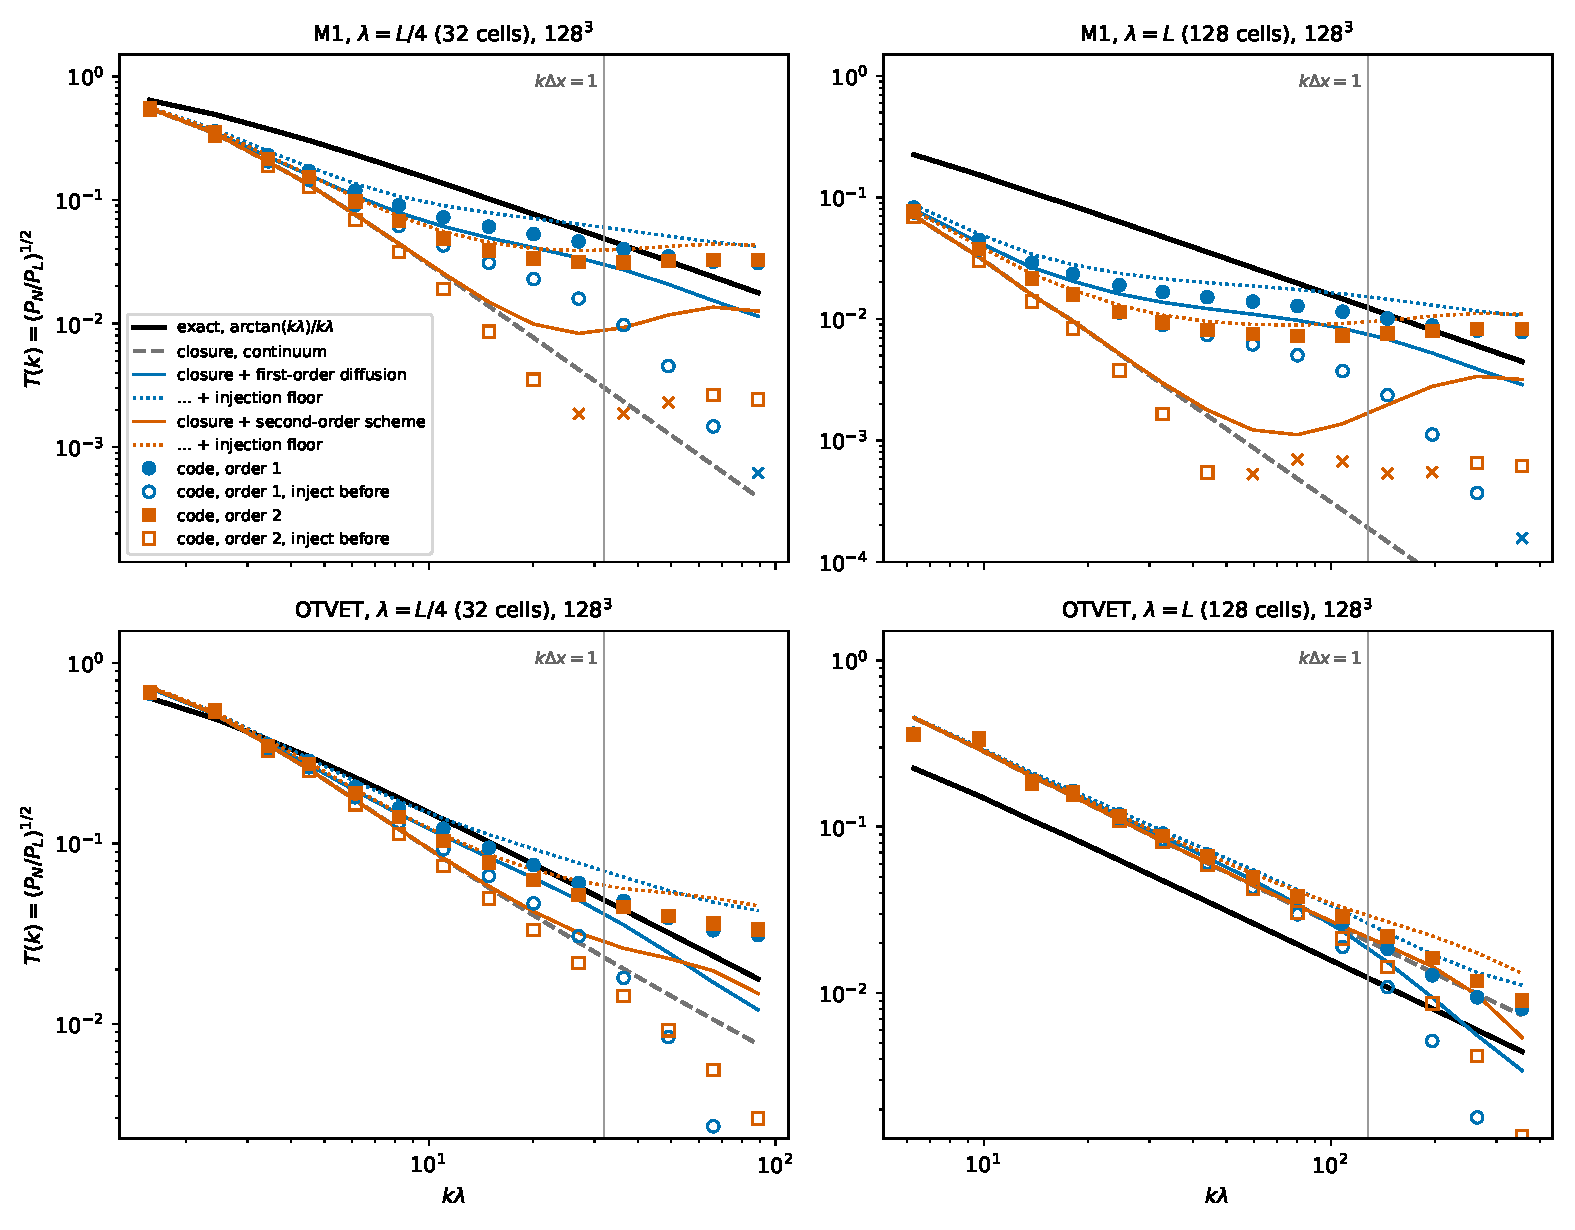
\includegraphics[width=\linewidth]{figures/convergence/fig_transfer_diffusion.pdf}
\caption{Transfer function between sources and photon density for a uniform mean free path, every cell a source, $128^3$
cells: M1 (top) and OTVET (bottom), $\lambda=L/4$ (left) and $\lambda=L$ (right). Black: the exact solution.
Grey dashed: the linear solution of the closure in the continuum. Thin solid lines: the same with the numerical
diffusion of the first-order (blue) and second-order (orange) scheme, equation (\ref{eq:glf}); dotted: with the
injection floor of equation (\ref{eq:floor}) added. Symbols: the code, first order (circles) and second order
(squares), with injection after (filled, the default) and before (open) the transport. Crosses: bins where the response is
less than 50\,\% correlated with the sources. The vertical line marks $k\dx=1$.}
\label{fig:transfer}
\end{figure}

Figure~\ref{fig:transfer} is the main result. Tables: \texttt{data/convergence/T\_N*.txt} and
\texttt{moment\_transfer\_order2.txt}.

\begin{itemize}
\item \textbf{Both solvers solve their equations.} At $k\lambda\lesssim2$ ($\lambda=L/4$) M1 is within
2--13\,\% and OTVET within 6\,\% of the continuum linear solution at every resolution from $32^3$ to
$256^3$. With every cell a source M1 equals the isotropic closure to four digits. For 30 sources in the box ($0.06$ per $\lambda^3$, $\lambda=L/8$), where each
cell holds one beam and M1 is exact, M1 follows the exact solution to 11\,\% over $k\lambda=2$--20.
\item \textbf{M1 with the default settings lies between the diffusion model and the model with the floor.}
The code (filled circles) is 1.0--1.4 times $T^{\rm GLF}_{\rm M1}$ at $k\dx<1$ and below the curve with the
floor, which overestimates it. It is 2.9 ($\lambda=L/4$) and 9.4 ($\lambda=L$) times the continuum M1 at $k\dx=0.34$, and 17 and 69 times at
$k\dx=1.1$.
\item \textbf{The agreement of M1 with the exact solution at short $\lambda$ is produced by these terms.} At
$\lambda=L/4$ the default M1 is within 0.5--1.0 of the exact solution up to $k\dx\approx1$ and crosses above
it at $k\dx\approx1.3$; the continuum M1 is 5--20 times below it there. The crossing is at the same
$k\dx$ at every resolution and every $\lambda$ tested: it is numerical. In equation
(\ref{eq:floor}), $T_1-T_0=f(1-T_0)$ holds to 1--4\,\% at $32^3$, $64^3$ and $128^3$.
\item \textbf{Injection before the transport removes the floor but smooths the sources.} With the first-order scheme
(open circles) M1 is 1.0--1.7 times the continuum up to $k\dx\approx0.3$ at $\lambda=L/4$. It lies below the
diffusion model, at 0.6--0.9 of it for $k\dx\le0.5$ and far below for $k\dx\gtrsim1$: the four subcycles spread a source's photons over about two cells before
the rate is evaluated. It never crosses the exact solution.
\item \textbf{The second-order scheme removes the diffusion term, not the floor.} With the default
injection (filled squares) it lowers M1's $T$ by a factor 1.1--1.9 at $k\dx=0.1$--0.8; what remains follows
the floor. With injection before the transport (open squares) the excess is gone and $T$ is 0.9 of the
continuum at $k\dx\le0.2$, but 0.3--0.8 at $k\dx=0.3$--0.5, below the linear model, and at $\lambda=L$ the
small residual response is anticorrelated with the sources for $k\dx=0.5$--1.1. The source field of this test
is white noise, the least favourable input for a slope limiter; the cause is not established.
\item \textbf{OTVET is insensitive at long $\lambda$ and M1-like at short $\lambda$.} At $\lambda=L$ its tensor
term dominates and the code is within 0.8--1.2 of its continuum solution at every resolution and either
order; it is 1.6--2.3 times the exact $T$. At $\lambda=L/4$ the tensor term is small, the solution is lifted by
the same two numerical terms as M1 (1.2--2.4 times its continuum at $k\dx=0.2$--1.1), and this brings it to
within 0.8--1.15 of the exact solution.
\end{itemize}

\subsection{Convergence with resolution}

\begin{figure}
\centering
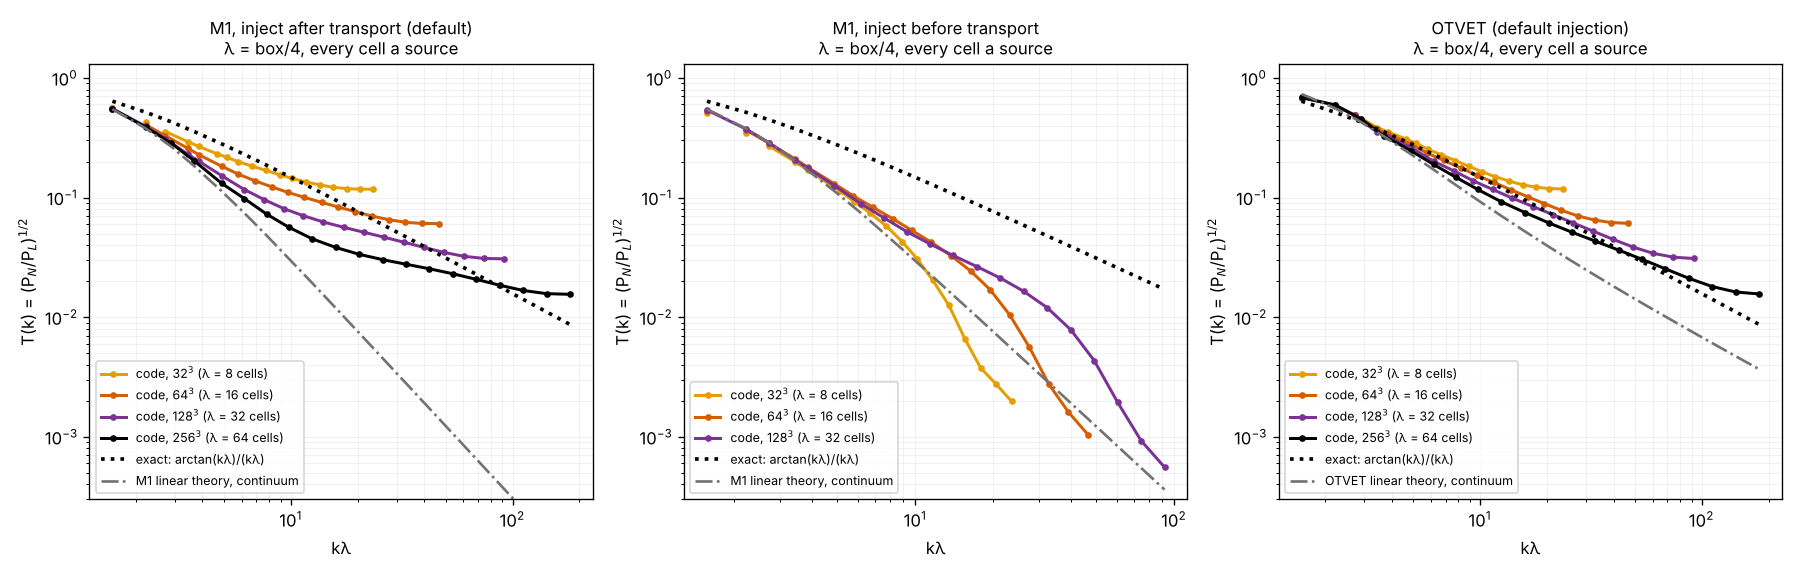
\includegraphics[width=\linewidth]{figures/convergence/moment_transfer_convergence_l4.png}
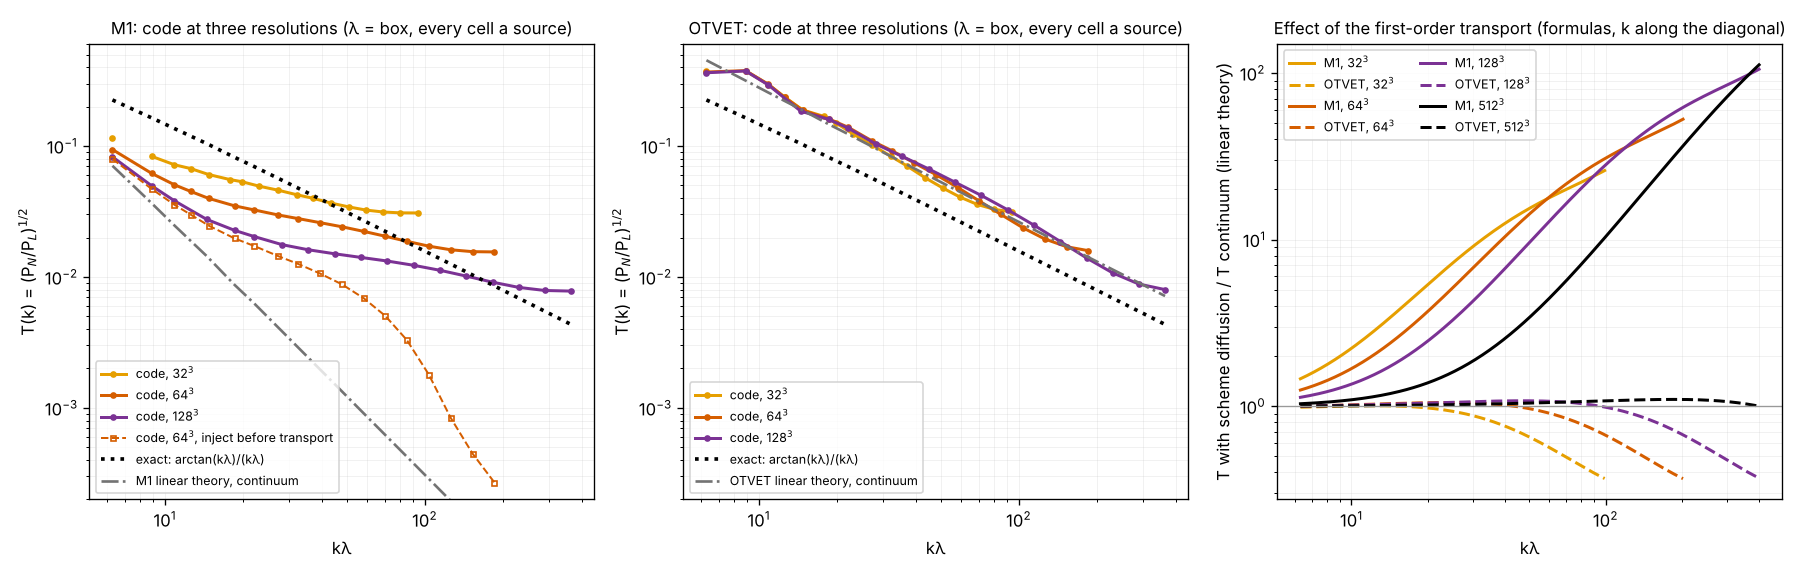
\includegraphics[width=\linewidth]{figures/convergence/moment_transfer_convergence.png}
\caption{The first-order scheme against resolution. Top: $\lambda=L/4$, $32^3$ to $256^3$: M1 with the default
injection (left), with injection before the transport (middle), and OTVET (right). Bottom: $\lambda=L$, $32^3$ to
$128^3$: M1 (left; open squares: injection before the transport at $64^3$), OTVET (middle), and the ratio of
equation (\ref{eq:glf}) to the continuum solution for modes along the diagonal (right).}
\label{fig:uniconv}
\end{figure}

\begin{table}
\centering
\caption{$T/T_{\rm continuum}$ of the closure at fixed $k\lambda$ in the uniform test, every cell a source,
interpolated in $\log k$ between the bins of \texttt{data/convergence/T\_N*.txt}. At $k\lambda=10$ and
$\lambda=L/4$, $k\dx=1.25$, 0.63, 0.31, 0.16 from $32^3$ to $256^3$.}
\label{tab:uniconv}
\begin{tabular}{llcccc}
\toprule
Case & $k\lambda$ & $32^3$ & $64^3$ & $128^3$ & $256^3$\\
\midrule
\multicolumn{6}{l}{$\lambda=L/4$}\\
M1, order 1 & 10 & 4.9 & 3.7 & 2.6 & 1.8\\
M1, order 2 & 10 & 4.4 & 2.6 & 1.8 & 1.4\\
M1, order 1 & 20 & 16 & 9.9 & 6.9 & 4.4\\
M1, order 2 & 20 & 17 & 8.4 & 4.4 & 2.7\\
M1, order 1, inject before & 10 & 1.09 & 1.72 & 1.60 & 1.34\\
M1, order 2, inject before & 10 & 0.56 & 0.63 & 0.79 & 0.89\\
OTVET, order 1 & 10 & 1.81 & 1.62 & 1.41 & 1.22\\
OTVET, order 2 & 10 & 1.85 & 1.43 & 1.22 & 1.11\\
OTVET, order 1 & 20 & 3.0 & 2.2 & 1.9 & 1.6\\
\midrule
\multicolumn{6}{l}{$\lambda=L$}\\
M1, order 1 & 25 & 9.9 & 6.3 & 3.8 & 2.4\\
M1, order 2 & 25 & 6.6 & 3.6 & 2.3 & 1.6\\
OTVET, order 1 & 25 & 1.05 & 1.09 & 1.07 & 1.04\\
OTVET, order 2 & 25 & 1.16 & 1.08 & 1.05 & 1.02\\
\bottomrule
\end{tabular}
\end{table}

\begin{itemize}
\item \textbf{M1 is not converged at any $k>1/\lambda$ with the default settings.} At fixed $k\lambda$ its $T$ falls
toward the continuum solution by a factor 1.35--1.65 per doubling of the resolution, somewhat slower than first order in
$\dx$, the scaling of both numerical terms (Table~\ref{tab:uniconv}).
\item The second-order scheme is a factor 1.2--1.7 closer to the continuum from $64^3$ up and converges
a little faster (1.3--2.0 per doubling). At $32^3$ and $\lambda=L/4$ it gains nothing: there $k\lambda\ge10$ is
$k\dx\ge1.25$. With injection before the
transport it approaches the continuum from below, 0.56, 0.63, 0.79, 0.89 from $32^3$ to $256^3$ at $k\lambda=10$.
\item OTVET is converged at $\lambda=L$ and converges like M1, with smaller amplitude, at $\lambda=L/4$.
\end{itemize}

\subsection{The same test with the rays}\label{sec:raytest}

\begin{figure}
\centering
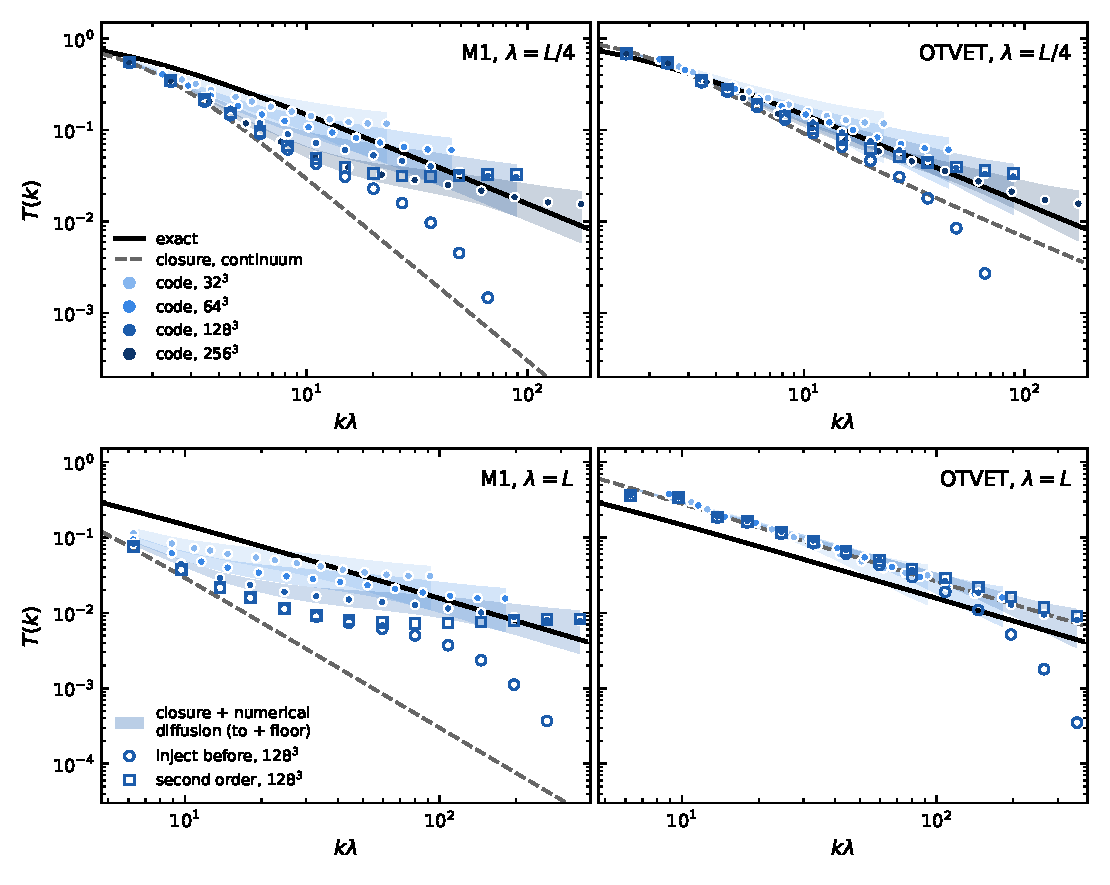
\includegraphics[width=\linewidth]{figures/fig_app_convergence.pdf}
\caption{The appendix figure of the paper: M1 (left) and OTVET (middle) as in Figs.~\ref{fig:transfer} and
\ref{fig:uniconv}, with the exact linear solution of the discrete scheme (Section~\ref{sec:disc}) as thin
curves; right, the ray tracer at $128^3$ for pools of 8, 15, 64 and 120 rays per cell (light to dark), with
$[T_{\rm exact}^2+\sigma^2/512]^{1/2}$, $\sigma=0.95\,n_{\rm ray}^{-1/2}$, as thin curves and the pool of 15
averaged over 16 substeps as open circles. Script: \texttt{scripts/fig\_app\_convergence.py --variants}.}
\label{fig:raytest}
\end{figure}

\paragraph{Set-up.} \texttt{tools/analysis/ray\_transfer.cpp} (branch \texttt{rt-convergence-runs}) runs the
solver's own ray tracing (thresholds, pool guard, emission, casting, splitting, merging and the deposit, then
the attenuation and the move) and replaces only the chemistry: every cell transmits $e^{-\dx/\lambda}$ of the
photons deposited in it, in every frequency group. The gas is made fully ionized, so the deposit is the path
share of a ray in each cell. $N$ is the photon count a cell holds in a substep, summed over the groups, which is
what the chemistry is given. A source cell emits 192 rays per substep, so a source in every cell is not
possible; the sources are $N^3/512$ random cells (4096 at $128^3$), a white field with
$P_L=512\,\dx^3\bar L^2$. The luminosity is set so that the mean is 0.1 photons per hydrogen atom per cell in
steady state (my estimate of the level in the suite after overlap; the ray deletion threshold $10^{-6}$ is
absolute). Runs last $20\lambda/\dx$ substeps, with the suite's settings otherwise (\texttt{legacy\_rt = 0},
\texttt{ray\_rotate = 3}). M1 and OTVET were run with the same source cells: their $T$ agrees with that for a
source in every cell to 4\,\% ($\lambda=L/4$) and 1\,\% ($\lambda=L$) in every bin, so the columns of
Fig.~\ref{fig:raytest} can be compared.

\paragraph{Result.} Table~\ref{tab:raytest} and Fig.~\ref{fig:raytest}. The transfer function separates into
a part correlated with the sources, $rT$ with $r$ the correlation coefficient, and an uncorrelated part
$T(1-r^2)^{1/2}$ (\texttt{scripts/ray\_noise.py}).
\begin{itemize}
\item \textbf{The correlated part is the exact solution.} $rT/T_{\rm exact}$ is 0.95--1.05 in every bin for
$\lambda=L/4$ at every pool size, and 0.87--1.09 for $\lambda=L$ (0.95--1.09 at $k\lambda>30$; the lowest
bins hold 6--20 modes). There is no diffusion plateau and no resolution-dependent floor: at the Nyquist
frequency $rT/T_{\rm exact}$ is 0.99--1.05 ($\lambda=L/4$) and 1.00--1.09 ($\lambda=L$). The rays do have an
injection term, since a substep's emission is deposited in and next to the source cell in that substep, but
it is the true one: these are the photons at $r<\dx$ of equation~(\ref{eq:exact}). A dip of 5\,\% at
$k\dx\approx1.5$--2 is the only systematic feature.
\item \textbf{The rest is white noise set by the number of rays per cell.} The uncorrelated part is flat in $k$
and corresponds to an rms per cell and substep of $\sigma=0.95\,n_{\rm ray}^{-1/2}$ of the mean (0.86--1.01
over the eight runs), close to the Poisson value for $n_{\rm ray}$ equal rays. For the suite's pool of 15,
$n_{\rm ray}=12.6$ and $\sigma=0.27$. In general $P_{\rm noise}=\sigma^2\dx^3\bar N^2$, that is
$\Delta^2_{\rm noise}(k)=\sigma^2(k\dx)^3/2\pi^2$, $1.6\,\sigma^2=0.11$ at the Nyquist frequency for the
suite. In units of $T$ the noise is $\sigma/\sqrt{512}$ in this test: its height relative to the signal in
Fig.~\ref{fig:raytest} is that of this source field, and it is larger at $\lambda=L$ only because the signal
is smaller.
\item \textbf{It averages down, but not as fast as independent draws.} Over 16 substeps $\sigma$ falls by 1.5
($\lambda=L/4$) and 2.5 ($\lambda=L$) at the pool of 15, against 4 for independent substeps: the same rays
persist from one substep to the next.
\item The pool guard limits the splitting in almost every substep at the pool of 15 (631 of 640 and 2551 of
2560) without a visible effect on the correlated part. At a pool of 8 it also forces merges, and 0.3\,\% of the
photons are lost at $\lambda=L$.
\item At $64^3$ and the pool of 15 the result is the same: $rT/T_{\rm exact}=0.95$--1.00 and $\sigma=0.20$
($\lambda=16$ cells), 0.87--1.18 and $\sigma=0.26$ ($\lambda=64$ cells).
\item Not varied: the source density, the mean photon count, and the number of merge directions.
\end{itemize}

\begin{table}
\centering
\caption{The rays in the uniform test at $128^3$. $T/T_{\rm exact}$ at the Nyquist frequency and the noise
per cell $\sigma$, for one substep and (in brackets) the mean of 16.}
\label{tab:raytest}
\begin{tabular}{llcccc}
\toprule
 & pool per cell & 8 & 15 (suite) & 64 (original) & 120\\
\midrule
$\lambda=L/4$ & rays per cell $n_{\rm ray}$ & 6.7 & 12.6 & 39.3 & 63.2\\
 & substeps limited / forced (of 640) & 318 / 314 & 631 / 0 & 12 / 0 & 0 / 0\\
 & $T/T_{\rm exact}$, Nyquist & 1.34 (1.13) & 1.21 (1.10) & 1.04 (1.01) & 1.02 (1.00)\\
 & $\sigma$ & 0.37 (0.23) & 0.26 (0.17) & 0.14 (0.09) & 0.11 (0.09)\\
 & $\sigma\,n_{\rm ray}^{1/2}$ & 0.96 & 0.91 & 0.90 & 0.86\\
\midrule
$\lambda=L$ & rays per cell $n_{\rm ray}$ & 6.7 & 12.6 & 31.2 & 52.1\\
 & substeps limited / forced (of 2560) & 1628 / 924 & 2551 / 0 & 11 / 0 & 0 / 0\\
 & $T/T_{\rm exact}$, Nyquist & 3.88 (1.58) & 2.77 (1.34) & 1.90 (1.19) & 1.56 (1.07)\\
 & $\sigma$ & 0.39 (0.16) & 0.28 (0.11) & 0.18 (0.08) & 0.14 (0.06)\\
 & $\sigma\,n_{\rm ray}^{1/2}$ & 1.01 & 0.97 & 0.98 & 0.97\\
\bottomrule
\end{tabular}
\end{table}

\subsection{Relation to Gnedin (2025) and to the suite}

\citet{gnedin25} finds that M1 and OTVET both follow $\arctan(k\lambda)/(k\lambda)$ in this test, with fitted
$\lambda\approx0.3$--$1\mpch$ in a $20\mpch$ box. The results above agree with his in that regime ($\lambda\ll L$)
and add two points. First, with many sources per $\lambda^3$ the agreement of M1 is produced by the numerical terms
and moves with resolution. Second, at $\lambda\gtrsim L$, the regime of our runs after overlap, the
closures depart from the exact solution in opposite directions: in power, M1 has 0.17 ($\lambda=L$) and 0.06
($\lambda=2.5L$) and OTVET 3--5 and 11--26 times the exact value at the box scale. The paper's $512^3$ suite at
$z=5$ has M1 at 0.04--0.07 and OTVET at 12--14 times the rays' $P_\Gamma$ at $k\le2\hmpc$: the suite's
post-overlap numbers are those of the closures at $\lambda\approx2.5L$. Which mechanism makes his runs agree
(few sources per $\lambda^3$, the numerical terms, or the shared ionized/neutral pattern during reionization)
is not established here.

%======================================================================
\section{Other tests of the moment solver}\label{sec:other}

\paragraph{Unit tests.} Photon and energy conservation of the transport to rounding; realizability; the
light-cone spread of a pulse; an M1 plane beam that moves exactly one cell per substep without sideways spread;
the OTVET tensor of a single source (rank one, unit trace, the periodic images) and the agreement of the
direct and FFT sums to $3\times10^{-7}$; redshifting of the group spectrum. Outputs are byte-identical for
1, 2 and 4 threads, and a restart from a checkpoint is bit-identical. For the second-order scheme: a point
pulse after five substeps has an rms width of 1.11 (M1) and 0.80 (OTVET) cells against 1.85 and 1.48 at first
order, and the $L_1$ error of a smooth advected wave falls by 3.6 per doubling of the resolution.

\paragraph{Photon budget.} In every run the photons injected, absorbed, lost to redshift and in flight
balance to six digits.

\paragraph{I-front in a uniform medium} ($32^3$, $\chat=0.1c$, one source). Photons emitted at $t'$ reach
a front of radius $R$ at $t'+R/\chat$, so the front is where the infinite-speed front $R_\infty$ was at the
retarded time,
\begin{equation}
R(t)=R_\infty\!\left(t-R(t)/\chat\right),\label{eq:ifront}
\end{equation}
which without recombinations ($R_\infty^3=3Qt$, $Q=\dot N_\gamma/4\pi n_{\rm H}$) is the solution of
Shapiro et al.\ (2006), $R^3/3+(Q/\chat)R=Qt$, with $R\to\chat t$ early and $R\to R_\infty$ late.
$R_\infty(t)$ is taken from the ray run at the full speed of light, corrected with the same relation, and
$\chat$ is the speed the code realises (one cell per substep); there is no free parameter. The radius is
$R=(3V_{\rm ion}/4\pi)^{1/3}$ with $V_{\rm ion}=\sum x_{\rm HII}$ over the cells. Error of the front radius
against equation (\ref{eq:ifront}):
\begin{center}
\begin{tabular}{lcccc}
\toprule
$\chat t$ [cells] & 2 & 6 & 10 & 30\\
\midrule
rays & $+1.9\,\%$ & $+3.8\,\%$ & $+1.7\,\%$ & $+0.2\,\%$\\
M1 & $+36\,\%$ & $+6.5\,\%$ & $+3.0\,\%$ & $+0.3\,\%$\\
OTVET & $+36\,\%$ & $+4.6\,\%$ & $+1.6\,\%$ & $-0.6\,\%$\\
M1, inject before & $+61\,\%$ & $+15\,\%$ & $+7.4\,\%$ & $+1.7\,\%$\\
OTVET, inject before & $+61\,\%$ & $+14\,\%$ & $+6.0\,\%$ & $+0.8\,\%$\\
\bottomrule
\end{tabular}
\end{center}
The moment fronts run ahead while they are a few cells across, because the first-order scheme carries
photons ahead of the light cone in the first substeps (the four subcycles reach four cells while light
travels one), and with injection before the transport because the source cell barely absorbs. They converge
to the solution once the front is resolved; the front stays about 1.5 times thicker than the rays'.

\paragraph{Shadow behind a dense clump} (a point-source test of our own). The mean ionized fraction on the
axis behind the clump is 0.000 for the rays, 0.044 for M1 and 0.004 for OTVET.

\paragraph{Two sources and 16 sources in a lognormal density field.} Two isotropic sources 12 cells apart give
the same ionized widths for the rays, M1 and OTVET. In the lognormal box at half ionization M1 and OTVET are
6\,\% and 3\,\% above the rays in ionized fraction (16\,\% and 11\,\% with injection before the transport), with
1.6 times as many partly ionized cells; 18--19\,\% of the cells differ from the rays by more than 0.1 in
$x_{\rm HII}$, against 6\,\% between two ray runs with different HEALPix frames.

\paragraph{Injection order and neutral source cells.} With injection before the transport, dense source cells stay
neutral however bright the source: at $512^3$ and $z=5.4$ M1 left 21\,\% of the cells at 100--500 times the mean
density neutral (rays 1.2\,\%, OTVET 2.3\,\%), with $\Gamma$ 500 times below their surroundings. Injection after
the transport lowers M1's residual neutral fraction after overlap by a factor 30--60, to the level of OTVET and of the rays,
and restores the proximity peaks ($\Gamma_{\rm max}$ 2--3 times the rays'). This is why it is the default, and why
the injection floor of Section~\ref{sec:uniform} is present in the suite. Section~\ref{sec:inject} gives the
dense-cell statistics of the convergence runs.

%======================================================================
\section{Reionization convergence runs}\label{sec:reion}

\subsection{Set-up}

The runs use the parameters of the paper's suite in a $20\mpch$ box with $512^3$ particles and a $512^3$ gravity mesh in every
run. The gas and radiation grid has $N^3=128^3$, $256^3$ or $512^3$ cells. The initial particle
data are byte-identical between resolutions. The suite ($40\mpch$, $512^3$ cells, $1024^3$ particles) has the cell
size and particle mass of the $256^3$ runs here; the $512^3$ runs have half the suite's cell.

\begin{itemize}
\item \textbf{Resolution series:} rays, M1, and OTVET at each $N$; M1 with injection before the transport
at every $N$; M1 and OTVET with the second-order scheme at $128^3$ and $256^3$.
\item \textbf{Ray-budget series} at $256^3$: the cap on rays per cell (\texttt{nray\_max\_factor}) $f=8$, 15
(the suite's value), 32, 64 and 120.
\item Spectra are of $\delta_\Gamma=\Gamma/\langle\Gamma\rangle_V-1$ and of $x_{\rm HII}$, compared at
matched ionized fraction $\xv$, because the histories differ between resolutions; after overlap at matched
redshift. $\lambda$ is the mean free path at 912\,\AA\ from the suite's estimator.
\end{itemize}

\paragraph{Caveats, stated plainly.}
\begin{itemize}
\item \textbf{The sources are not matched between resolutions.} Halo counts at fixed redshift differ by about
$-26\,\%$ ($128^3$) and $+14$ to $+32\,\%$ ($512^3$) relative to $256^3$, and the total luminosity by up to
30\,\% at $z>11$ and 2--4\,\% below $z=9$. The likely cause, not tested, is the gas's gravity being smoothed on the
coarser gas grid.
\item \textbf{The $512^3$ runs do not reach overlap} by $z=5$ (rays: $\xv=0.84$ at $z=4.97$; M1: 0.87). The
after-overlap comparison exists only at $128^3$ and $256^3$.
\item \textbf{At $128^3$ the suite's ray budget fails.} With $f=15$ the ray pool filled (splitting limited
in 767 substeps and none from $\xv\approx0.75$). The $128^3$ reference is therefore an $f=120$ run. At
$256^3$ and $512^3$ the pool guard never triggered with $f=15$.
\item The gas resolution changes the absorbers. After overlap the $128^3$ rays have $\lambda=38$\,pMpc
against 15.5\,pMpc at $256^3$, and a quarter of the $\Gamma$ power at all $k$. This is the absorber
population, not the transport.
\item Snapshots of different runs are not at identical redshifts. Where they differ by $\Delta z\approx0.03$--0.05
the cross-correlation at $k\gtrsim8\hmpc$ drops (to 0.5--0.8 at $512^3$) and recovers to 0.96--0.99 where they
match.
\end{itemize}

\subsection{M1 and OTVET against the rays with resolution}

\begin{figure}
\centering
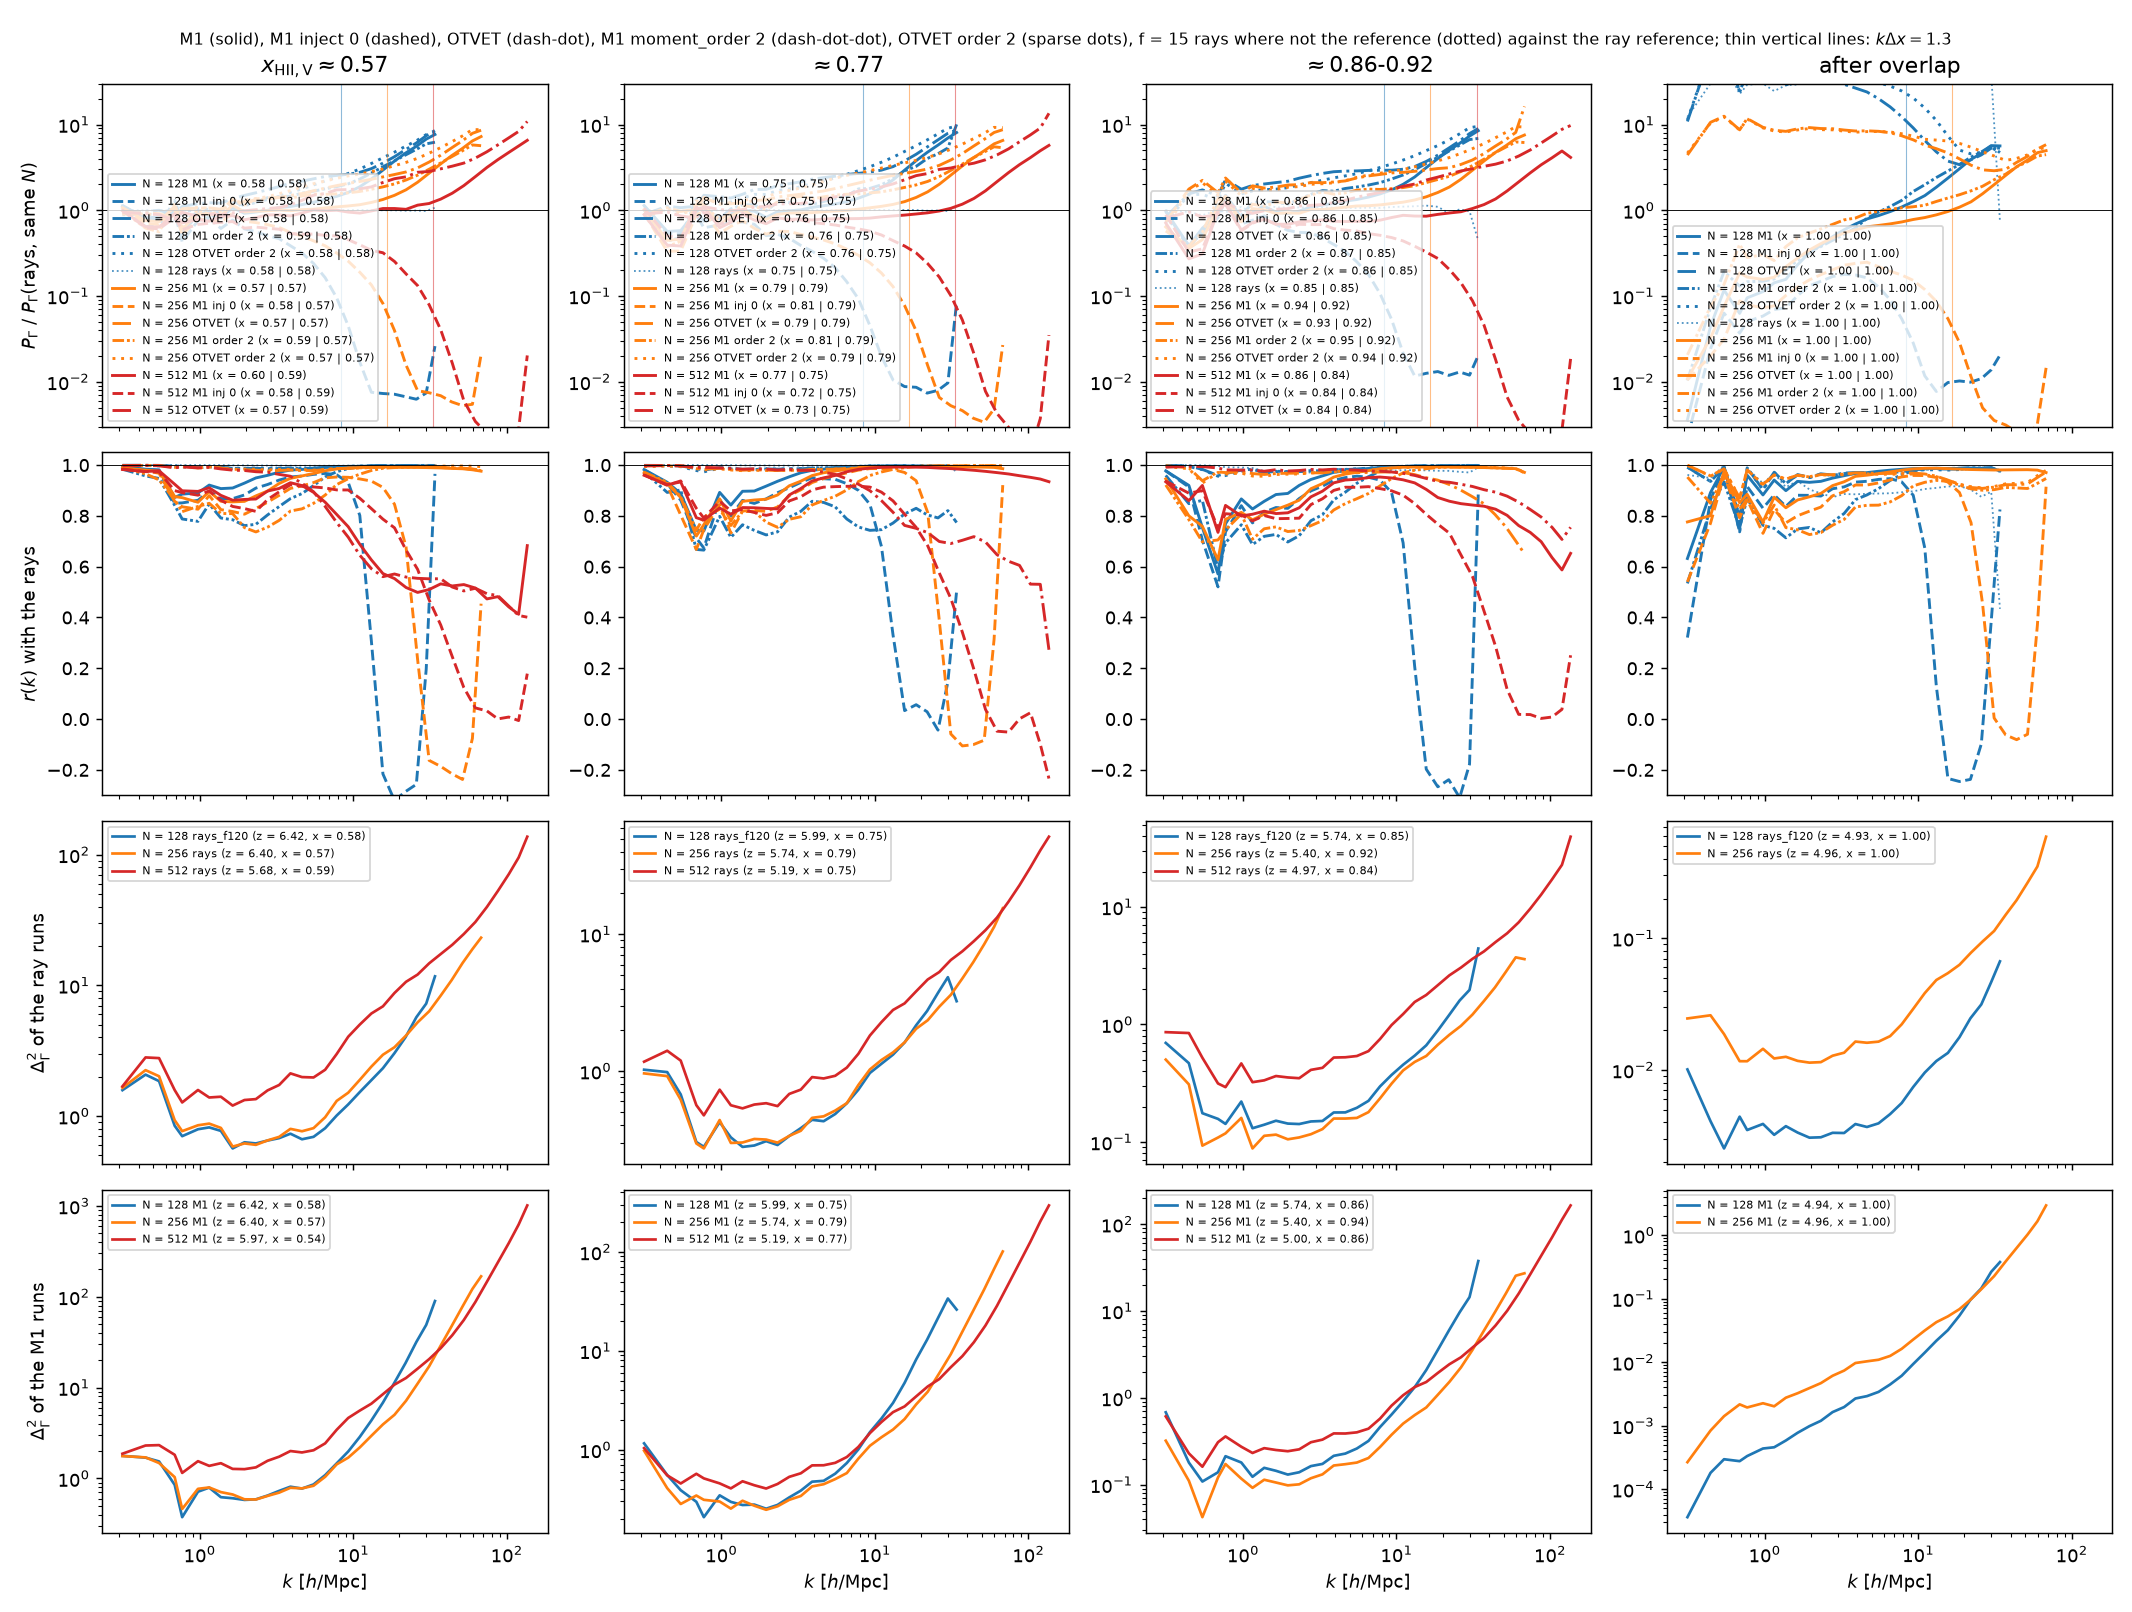
\includegraphics[width=\linewidth]{figures/convergence/rt_convergence_res.png}
\caption{Resolution series. Columns: $\xv\approx0.57$, 0.77, 0.86--0.92 and after overlap. Top: $P_\Gamma$ of
each moment run over that of the ray run with the same $N$ (blue $128^3$, orange $256^3$, red $512^3$; M1 solid, M1 with
injection before the transport dashed, OTVET dash-dotted, M1 second order dash-dot-dotted, OTVET second order
sparse dots); thin vertical lines: $k\dx=1.3$.
Second row: cross-correlation with the rays. Third and fourth rows: $\Delta^2_\Gamma$ of the ray runs and of the M1
runs themselves. Table: \texttt{data/convergence/rt\_convergence\_res.txt}.}
\label{fig:res}
\end{figure}

\begin{table}
\centering
\caption{$P_\Gamma({\rm M1})/P_\Gamma({\rm rays})$ at the same $N$ and matched $\xv$ (default settings).}
\label{tab:m1res}
\begin{tabular}{llccccc}
\toprule
Epoch & $N$ & $k=1$ & 2 & 4 & 8 & $16\hmpc$\\
\midrule
$\xv\approx0.57$ & 128 & 0.91 & 0.93 & 1.12 & 1.47 & 3.05\\
 & 256 & 0.91 & 0.96 & 0.99 & 1.10 & 1.36\\
 & 512 & 0.78 & 0.78 & 0.87 & 0.99 & 1.05\\
$\xv\approx0.77$ & 128 & 0.83 & 0.84 & 1.09 & 1.41 & 3.05\\
 & 256 & 0.71 & 0.80 & 0.94 & 1.04 & 1.28\\
 & 512 & 0.64 & 0.71 & 0.77 & 0.80 & 0.88\\
after overlap & 128 & 0.12 & 0.33 & 0.71 & 1.11 & 2.47\\
 & 256 & 0.16 & 0.35 & 0.60 & 0.74 & 0.98\\
\bottomrule
\end{tabular}
\end{table}

\begin{itemize}
\item \textbf{M1's small-scale excess is numerical and falls with resolution.} At $k=16\hmpc$ the ratio
goes $3.05\to1.36\to1.05$ ($\xv\approx0.57$) and $2.47\to0.98$ (after overlap) per doubling of $N$: a factor
2.2--2.5 from $128^3$ to $256^3$ and 1.3--1.5 from $256^3$ to $512^3$ (Table~\ref{tab:m1res}).
\item \textbf{After overlap M1 overtakes the rays at fixed $k\dx$,} 1.08 ($128^3$) and 1.28 ($256^3$), as the
uniform test predicts ($\approx1.3$). Before overlap the crossing is at $k\dx\approx0.2$--0.5, and at $512^3$ it moves from $k\dx=0.2$
($\xv\approx0.6$) to 1.1 ($\xv\approx0.75$).
\item \textbf{M1's large-scale deficit after overlap does not converge away:} 0.12 and 0.16 at $k=1\hmpc$,
0.33 and 0.35 at $k=2\hmpc$ at $128^3$ and $256^3$. This is the closure (Section~\ref{sec:uniform}).
\item \textbf{During reionization M1 moves below the rays with resolution} at $k=1$--$8\hmpc$: at
$\xv\approx0.77$ the ratio at $k=4\hmpc$ is 1.09, 0.94, 0.77. Part of this is the rays themselves: the $512^3$ ray run has
1.7--2.6 times the $\Gamma$ power of the $256^3$ one at $k\ge1\hmpc$ at the same $\xv$ (third row of
Fig.~\ref{fig:res}), reached at lower redshift.
\item \textbf{OTVET has more small-scale power than the rays at every resolution} during reionization, and the
excess shrinks slowly: at $\xv\approx0.57$, $P_\Gamma/P_\Gamma({\rm rays})$ at $k=2$, 4, 8, $16\hmpc$ is
1.50, 2.08, 2.56, 3.64 at $128^3$ and 1.27, 1.50, 1.96, 2.47 at $256^3$; at $512^3$ it is
0.99, 1.18, 1.73, 2.14 ($\xv\approx0.58$; 1.12, 1.26, 1.69, 2.30 at $\xv\approx0.74$). From $256^3$ to
$512^3$ the excess at fixed $k\ge8\hmpc$ falls by only 10--15\,\%. Its cross-correlation with the rays is
0.98--1.00 at $128^3$ and $256^3$ and 0.95--0.99 at $k\le4\hmpc$ at $512^3$, where at $k\ge8\hmpc$ it follows
the redshift mismatch of the paired snapshots as for M1.
\item \textbf{OTVET's excess after overlap is large and grows as the mean free path does:} 8--12 times the
rays' power at $k=0.5$--$4\hmpc$ at $256^3$ ($\lambda=15$--20\,pMpc) and 26--85 times at $128^3$
($\lambda=38$\,pMpc), in line with the $\lambda/L$ scaling of its tensor term.
\item \textbf{Second-order M1 in a reionization run does not reduce the excess, at $128^3$ or $256^3$.} At
$128^3$ the ratio to the rays
at $k=2$, 4, 8, $16\hmpc$ is 1.14, 1.47, 1.91, 3.29 at $\xv\approx0.58$ against 0.93, 1.12, 1.47, 3.05 at first order, and the
cross-correlation at $k=1$--$4\hmpc$ falls from 0.89--0.98 to 0.76--0.87. At $256^3$ it is 1.17, 1.40, 1.56, 1.90
against 0.96, 0.99, 1.10, 1.36, and the correlation falls from 0.86--0.95 to 0.75--0.84. After overlap at $256^3$
the second-order run has more power at every $k$: 0.30, 0.55, 0.83, 1.07, 1.41 of the rays' at $k=1$, 2, 4, 8,
$16\hmpc$ against 0.16, 0.35, 0.60, 0.74, 0.98, with a lower correlation (0.73--0.84 against 0.79--0.96 at
$k=1$--$4\hmpc$). The uniform test predicted a modest
reduction of the small-scale power. The cause is not known. It is not the build: a control run of the first-order scheme with the executable
of the second-order run reproduces the original first-order run byte for byte.
\item \textbf{Second-order OTVET does not reduce the excess either.} At $128^3$ it has less excess at
$k\le4\hmpc$ and more at $k=16\hmpc$: 1.21, 1.64,
2.47, 4.18 at $k=2$, 4, 8, $16\hmpc$ and $\xv\approx0.58$ against 1.50, 2.08, 2.56, 3.63 at first order, with the
same correlation with the rays (0.99). After overlap its excess at $k=4$--$16\hmpc$ is larger (33, 24, 7.0 against
26, 12, 3.7 times the rays). At $256^3$ it has more excess at every $k\ge1\hmpc$ during reionization: 1.33, 1.72,
2.38, 3.07 at $\xv\approx0.57$ against 1.27, 1.50, 1.96, 2.47, with the same correlation (0.98--0.99). After
overlap it is within 3\,\% of first order at $k\le4\hmpc$ (9.0, 9.0, 8.2 times the rays at $k=1$, 2, $4\hmpc$ against 9.2, 9.2,
8.4) and larger at $k=8$ and $16\hmpc$ (7.7 and 6.4 against 7.3 and 4.6).
\end{itemize}

\subsection{Injection before the transport in the reionization runs}\label{sec:inject}

\begin{itemize}
\item With injection before the transport M1 stays below the rays at every $k\ge0.5\hmpc$ and every epoch, and
falls to 0.01--0.1 of the rays' power at $k\dx\gtrsim1$ (Fig.~\ref{fig:res}, dashed). At $256^3$ and
$\xv\approx0.57$ the ratio is 0.79, 0.74, 0.54, 0.31 at $k=1$, 2, 4, $8\hmpc$, against 0.91, 0.96, 0.99, 1.10 with
the default. The difference between the two is the injection floor: most of M1's power above $k\approx4\hmpc$ at
$256^3$ is the source cells' own photons.
\item Its ratio depends on resolution as much as the default's does at fixed $k$, because the source smoothing is
also fixed in cells. At $\xv\approx0.58$ the ratio at $k=8\hmpc$ is 0.09, 0.31, 0.49 and at $k=16\hmpc$ 0.01, 0.07,
0.31 from $128^3$ to $512^3$: it approaches the rays from below, as in the uniform test. At $k=2\hmpc$ it is
0.60, 0.74, 0.62, with no trend.
\item At $512^3$ and $\xv\approx0.58$ the ratio is 0.69, 0.62, 0.53, 0.49, 0.31 at $k=1$, 2, 4, 8, $16\hmpc$,
against 0.78, 0.78, 0.87, 0.99, 1.05 with the default. The run reionizes earlier than the default: $\xv=0.954$ at
$z=4.98$, against 0.865 (default, $z=5.00$) and 0.837 (rays, $z=4.97$). Its dense-cell statistics were not computed.
\item \textbf{Dense cells} (more than 100 times the mean density) after overlap at $256^3$: mass-weighted neutral
fraction 0.110 (rays), 0.184 (M1) and 0.308 (M1, injection before); mean $\Gamma$ in those cells $3.6\times10^{-12}$,
$4.5\times10^{-12}$ and $7.4\times10^{-13}\,{\rm s^{-1}}$. At $128^3$: 0.028, 0.134 and 0.295. Injection before the
transport starves the densest cells of photons, as in Section~\ref{sec:other}.
\item The pre-overlap conclusions for M1 carry over to OTVET in the uniform test: with injection before the
transport OTVET is within 0.93--1.25 of its continuum solution up to $k\dx\approx0.7$, and the floor accounts for 65--80\,\%
of its excess. No OTVET reionization run with injection before the transport was made.
\end{itemize}

\subsection{Do the rays change with resolution?}

Yes, through the gas and the absorbers rather than the ray transport. At matched $\xv\approx0.57$--0.77 the $128^3$
and $256^3$ ray runs agree in $P_\Gamma$ to 10\,\% at $k\le4\hmpc$; the $512^3$ run has 1.3--2.6 times more
power at $k\ge0.5\hmpc$, a lower median $\Gamma$ in ionized gas ($2.4\times10^{-14}$ against $5.3\times10^{-14}\,{\rm s^{-1}}$) and a
later reionization. After overlap the $128^3$ run has $\lambda=38$\,pMpc and 73 cells above 100 times the mean density,
the $256^3$ run 15.5\,pMpc and 1500. The absolute $\Gamma$ statistics are therefore not converged in gas
resolution at the suite's cell size; the comparison between methods at fixed resolution is the robust quantity.

\subsection{Ray budget}

\begin{figure}
\centering
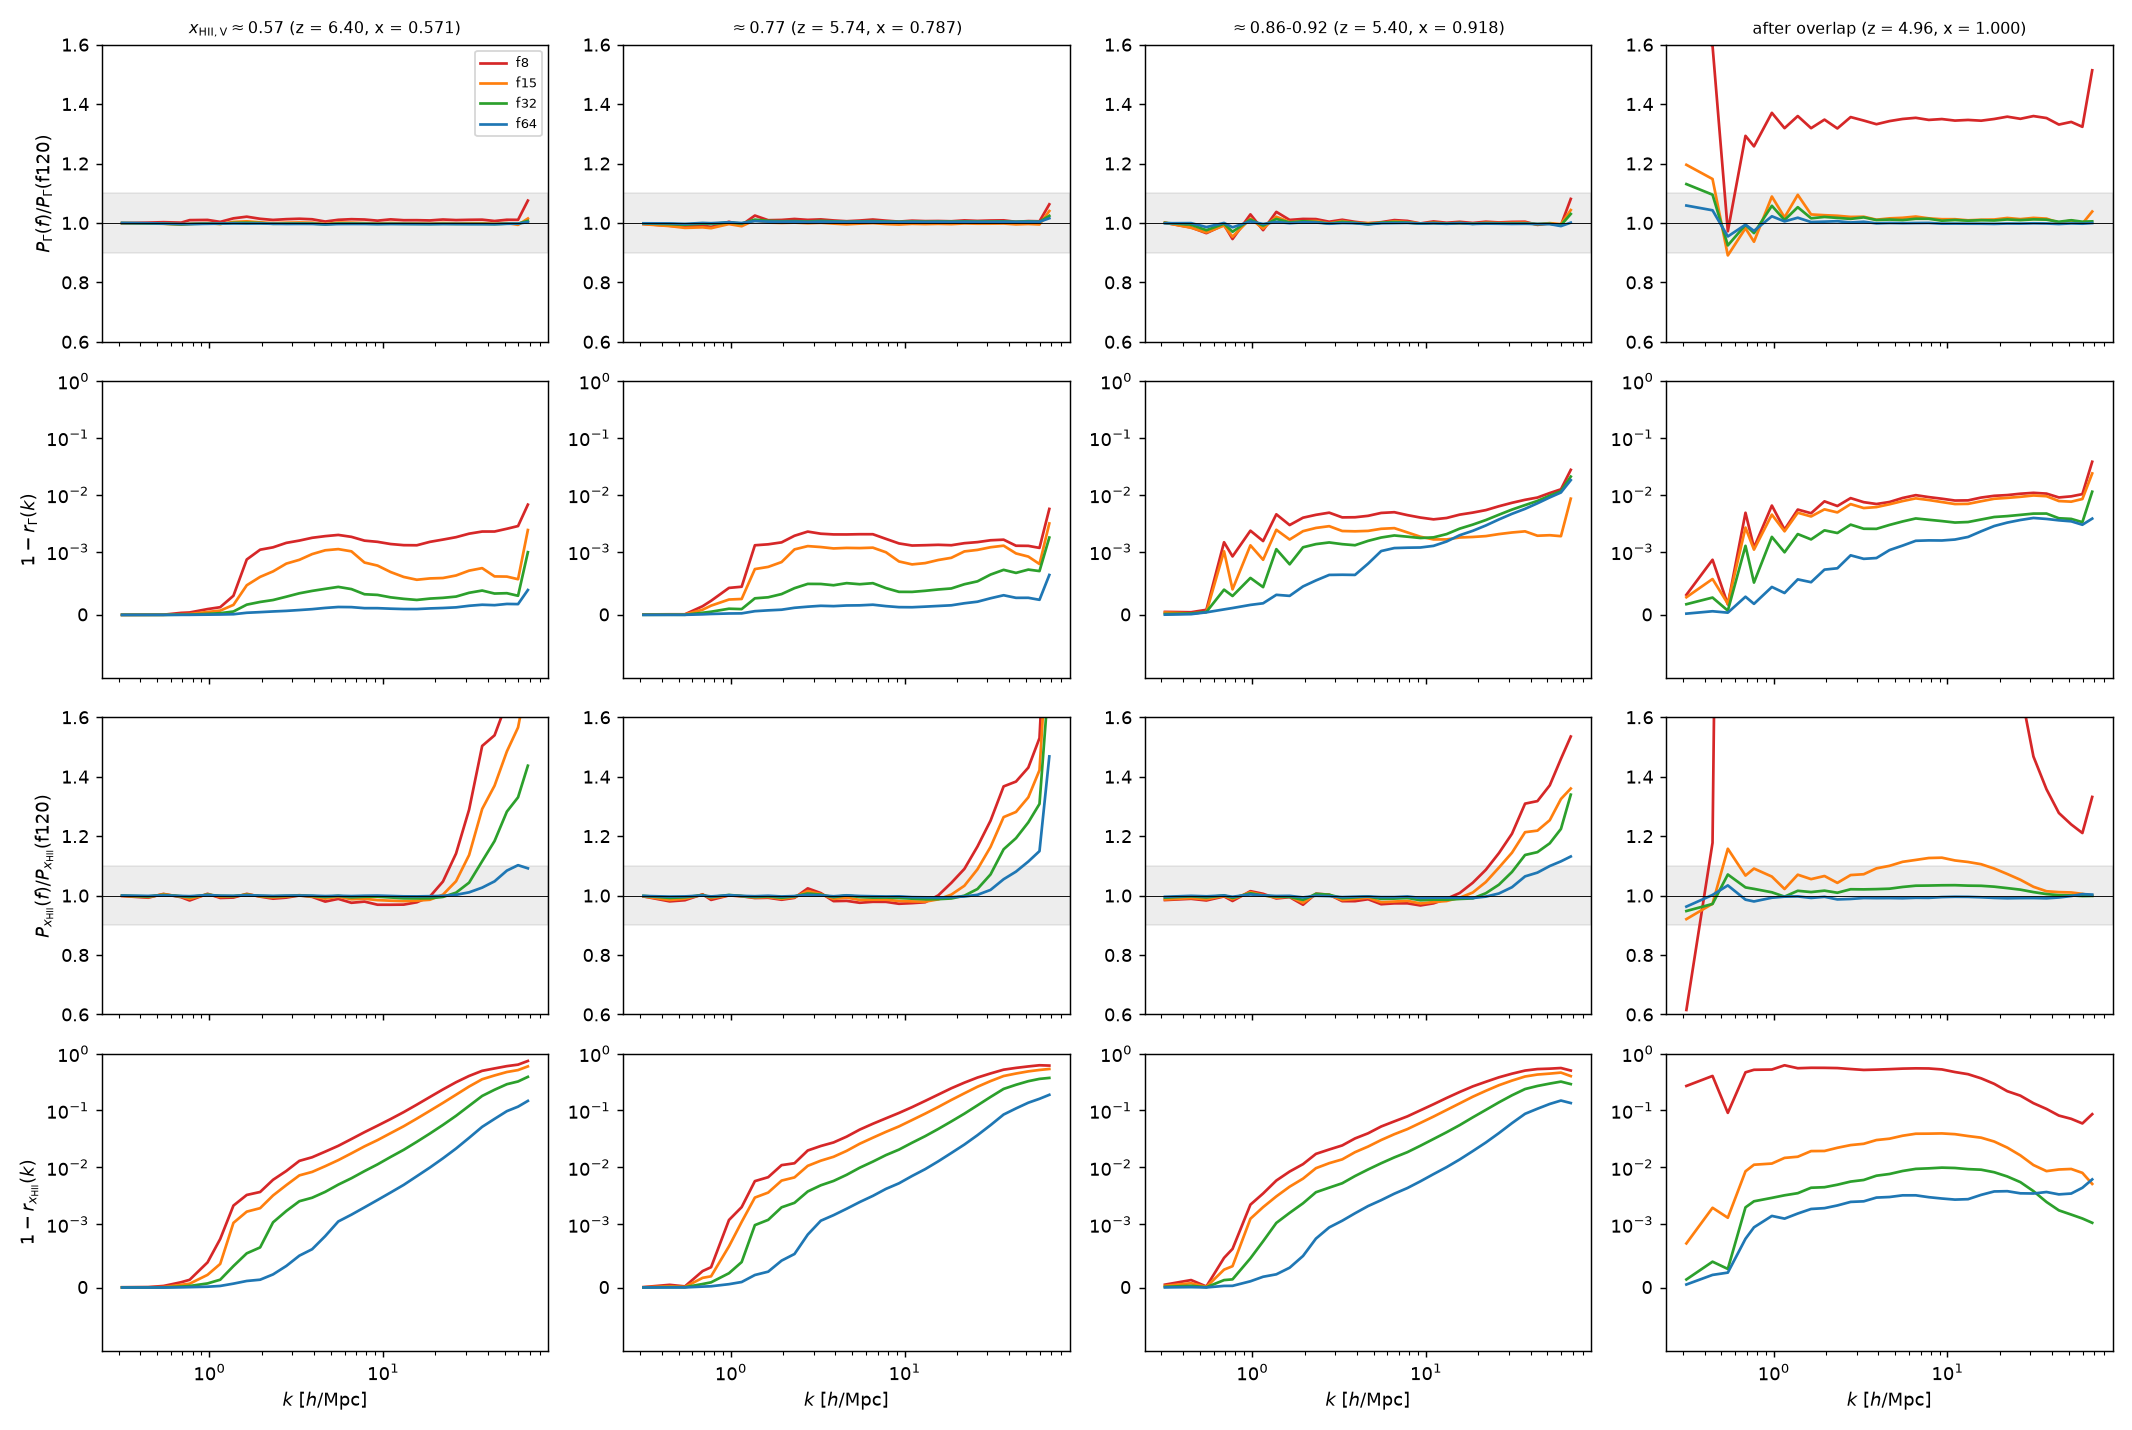
\includegraphics[width=\linewidth]{figures/convergence/rt_convergence_rays.png}
\caption{Ray-budget series at $256^3$: ratio of the power of $\Gamma$ and of $x_{\rm HII}$ to the $f=120$ run and
cross-correlation with it. Table: \texttt{data/convergence/rt\_convergence\_rays.txt}.}
\label{fig:rays}
\end{figure}

\begin{table}
\centering
\caption{Ray-budget runs at $256^3$ after overlap ($z=4.96$).}
\label{tab:rays}
\begin{tabular}{lccccc}
\toprule
 & $f=8$ & 15 (suite) & 32 & 64 & 120\\
\midrule
live rays per cell & 6.8 & 10.1 & 17.4 & 26.5 & 41\\
peak memory [GB] & 55 & 60 & 70 & 84 & 106\\
pool guard (substeps with splitting limited) & 1920 & 0 & 0 & 0 & 0\\
$\lambda$ [pMpc] & 12.7 & 15.5 & 15.8 & 16.0 & --\\
$P_\Gamma/P_\Gamma(f=120)$, $k=0.3\hmpc$ & 1.65 & 1.20 & 1.13 & 1.06 & 1\\
\quad $k=1\hmpc$ & 1.36 & 1.08 & 1.05 & 1.02 & 1\\
\quad $k=2\hmpc$ & 1.34 & 1.03 & 1.02 & 1.00 & 1\\
\quad $k=16\hmpc$ & 1.34 & 1.01 & 1.01 & 1.00 & 1\\
\bottomrule
\end{tabular}
\end{table}

\begin{itemize}
\item \textbf{During reionization the suite's budget is converged.} At $\xv\le0.92$ the $f=15$ run is within
5\,\% of $f=120$ in $P_\Gamma$ at every $k$ up to $68\hmpc$ (within 2\,\% at $\xv\le0.79$), with $r\ge0.99$.
\item \textbf{After overlap it is converged to 3\,\% at $k\ge2\hmpc$, 8\,\% at $k=1\hmpc$ and 20\,\% in the lowest
bin} ($k=0.3\hmpc$). The largest deviation at $k\le2\hmpc$ grows with the mean free path: 0.6\,\%, 2\,\%, 5\,\%, 20\,\%
at $\lambda=0.22$, 0.83, 2.1 and 16\,pMpc. The error is an excess of large-scale power.
\item $f=64$ and $f=120$ differ by at most 6\,\% (lowest bin) and 2\,\% elsewhere. $f=8$ is not usable after
overlap (35\,\% high, $\lambda$ 20\,\% short, pool guard active).
\item The power of $x_{\rm HII}$ after overlap (the residual neutral gas) is up to 13\,\% high at $f=15$.
\item Not varied: the number of merge directions per cell (\texttt{nside\_merge}), which would be the next test.
\item The $512^3$ ray run of this series ($f=15$) took 16.8\,h on 192 cores with a peak memory of 196\,GB and no pool-guard
events; the $256^3$ $f=15$ and $f=120$ runs took 2.5\,h and 7.5\,h.
\end{itemize}

\subsection{Cost of the rays against the moments}\label{sec:cost}

\begin{table}
\centering
\caption{Wall time of the reionization runs of this series (192 cores, to $z\approx5$), from the totals and the
RT timers at the end of each \texttt{run.log} and the live ray counts of \texttt{Log/ray.log}. Transport: the ray
tracing or the moment transport without the chemistry. The $512^3$ runs take 72--74 hydro steps, the others 48--49.}
\label{tab:cost}
\begin{tabular}{lccc}
\toprule
 & $128^3$ & $256^3$ & $512^3$\\
\midrule
total, rays [s] & 2370 & 9003 & 60\,537\\
total, M1 [s] & 571 & 3562 & 32\,123\\
total, OTVET [s] & 572 & 3606 & 32\,247\\
rays / M1, total & 4.1 & 2.5 & 1.9\\
RT, rays [s] & 1936 & 7787 & 53\,499\\
RT, M1 [s] & 255 & 3118 & 30\,026\\
rays / M1, RT & 7.6 & 2.5 & 1.8\\
transport, rays [s] & 1480 & 6091 & 40\,333\\
transport, M1 [s] & 146 & 1762 & 15\,972\\
rays / M1, transport & 10.1 & 3.5 & 2.5\\
chemistry, rays [s] & 92 & 1224 & 11\,896\\
chemistry, M1 [s] & 96 & 1255 & 12\,950\\
chemistry / RT, rays & 5\,\% & 16\,\% & 22\,\%\\
mean live rays per cell (end of run) & 9.3 (12.0) & 7.8 (10.1) & 5.0 (7.5)\\
source cells at the end & 33\,464 & 36\,758 & 41\,279\\
peak memory, rays / M1 / OTVET [GB] & 32 / 30 / 30 & 60 / 48 / 49 & 196 / 130 / 136\\
\bottomrule
\end{tabular}
\end{table}

The ratio of wall times falls with resolution because the cost of the rays follows their number and that of M1
the number of cells. The source cells are nearly the same at every resolution and each emits 192 rays per substep:
about 2.5 new rays per cell and substep at $128^3$ and 0.06 at $512^3$. At $128^3$ the pool is saturated (the
guard forced merges in 900 substeps); at $512^3$ it never fills. The chemistry is the same routine in both and
scales with the cells. The transport time per live ray and substep is about three times higher at $128^3$ than at
$256^3$ and $512^3$; the cause was not isolated. The trend is one of cell size at fixed box and sources: a larger
box at the same cell size has proportionally more sources. Not measured: either method beyond one node.

%======================================================================
\section{What was and was not run}\label{sec:status}

\begin{itemize}
\item Uniform test: first order at $32^3$--$256^3$ ($\lambda=L/4$ and $\lambda=L$), plus
$\lambda=L/8$ and $2.5L$ with few and many sources; both orders and both injection orders at $64^3$ and $128^3$.
The second order at $32^3$ and $256^3$ (both $\lambda$) is done.
\item Uniform test with the rays (Section~\ref{sec:raytest}): $128^3$ at pools of 8, 15, 64 and 120 per cell and
$64^3$ at 15, $\lambda=L/4$ and $L$, with M1 and OTVET on the same source cells.
\item Reionization runs finished: rays, M1 at $128^3$, $256^3$, $512^3$; OTVET at $128^3$, $256^3$, $512^3$; M1 with injection before the transport at $128^3$,
$256^3$ and $512^3$; the ray budgets; M1 and OTVET second order at $128^3$ and $256^3$.
\item Not run: OTVET with injection before the transport in a reionization
run; any $512^3$ run past overlap; the screen and cone closures in any of these tests; an HLL flux; the second-order scheme on refined grids.
\end{itemize}

\section{Suggested wording for the paper}

For ``Shared limitations'' in the main text, if the reionization runs are not shown:

\begin{quote}
Our M1 solver uses a first-order flux and deposits each source's photons in its own cell before
transporting them. In a medium of uniform mean free path these two choices set M1's response below a few cells
(Appendix~X): it exceeds the exact solution for $k\dx\gtrsim1.3$ and converges to the closure's own solution only
at first order in the cell size. In reionization runs at fixed box size the ratio of M1's $P_\Gamma$ to the rays'
at $k=16\hmpc$ falls from 3.1 to 1.4 to 1.05 as the grid goes from $128^3$ to $256^3$ to $512^3$ cells
(at $\xv\approx0.6$), a factor of about 2.3 and 1.3 per doubling, while at $k\le2\hmpc$ after overlap it stays at 0.1--0.35.
M1's excess small-scale power in Fig.~Y is therefore numerical, and its deficit at large scales is the closure.

The ray tracing caps the number of rays per cell. Raising the cap eightfold changes $P_\Gamma$ by less than 5\,\%
at all $k$ during reionization. After overlap our runs are converged to 3\,\% for $k\ge2\hmpc$ and overestimate the
power by 8\,\% at $k=1\hmpc$ and 20\,\% at $k=0.3\hmpc$.
\end{quote}

\bibliographystyle{aasjournal}
\bibliography{refs}

\end{document}
